\begin{figure}[h] 
\centering 
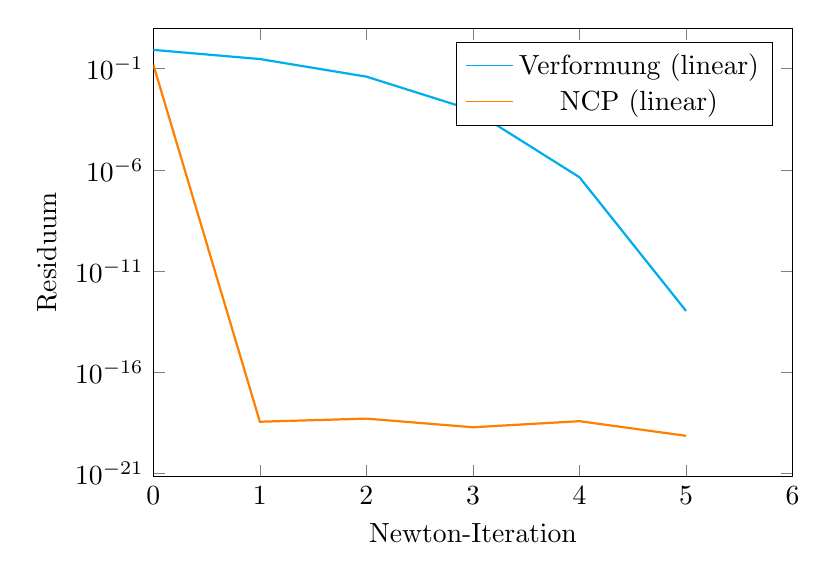
\begin{tikzpicture}[every plot/.append style={thick}] 
\begin{axis}[ 
label style={font=\normalsize}, 
xlabel={Newton-Iteration}, 
ylabel={Residuum}, 
xmin=0, xmax=6, 
ymode=log, 
ymin=0, ymax=10, 
width=0.8\textwidth, 
height=0.6\textwidth, 
legend pos=north east, 
legend style={cells={align=left}}, 
grid style=dashed, 
] 
\addplot[ 
color=cyan, 
] 
coordinates { 
(0, 8.51e-01)(1, 3.00e-01)(2, 4.05e-02)(3, 8.85e-04)(4, 4.31e-07)(5, 1.07e-13)}; 
\addlegendentry{Verformung (linear)} 
\addplot[ 
color=orange, 
] 
coordinates { 
(0, 1.60e-01)(1, 3.57e-19)(2, 5.09e-19)(3, 1.90e-19)(4, 3.80e-19)(5, 7.20e-20)}; 
\addlegendentry{NCP (linear)} 
\end{axis} 
\end{tikzpicture} 
\caption{Residuen des Stoffgesetzes 'Neo Hooke' mit Hinderniss 'Spitze' und 8450 Freiheitsgraden für die Verschiebung.} 
\label{fiq:NeoHooke_Spitze_level5} 
\end{figure} 
